\section{Experiments}
\label{sec:experiments}

Three levels of evidence. Policies small enough to enumerate, where the objective, the Fisher
information, the drift and both noise terms are computed rather than estimated. Transformers trained
from scratch, where a population of independent runs executes as one batched kernel so that sweeps
carry standard errors rather than anecdotes. And a pretrained model, where the same measurement is
made on a real policy and a real verifier. Everything ran on a single Apple M4 laptop.

\subsection{Seeds reconverge}
\label{sec:exp-seeds}

A population of transformers is warmed up, given identical parameters, and then trained with each
member drawing its own rollouts. Members differ in nothing else: same prompts corpus, same
objective, same schedule. Divergence is the mean KL between members' policies on a shared batch of
prompts, and outcome spread is the standard deviation of their pass rates, corrected for the
binomial error of the evaluation itself, which at the sample counts normally used accounts for most
of the raw spread and has to be removed before anything can be seen.

\begin{figure*}[t]
  \centering
  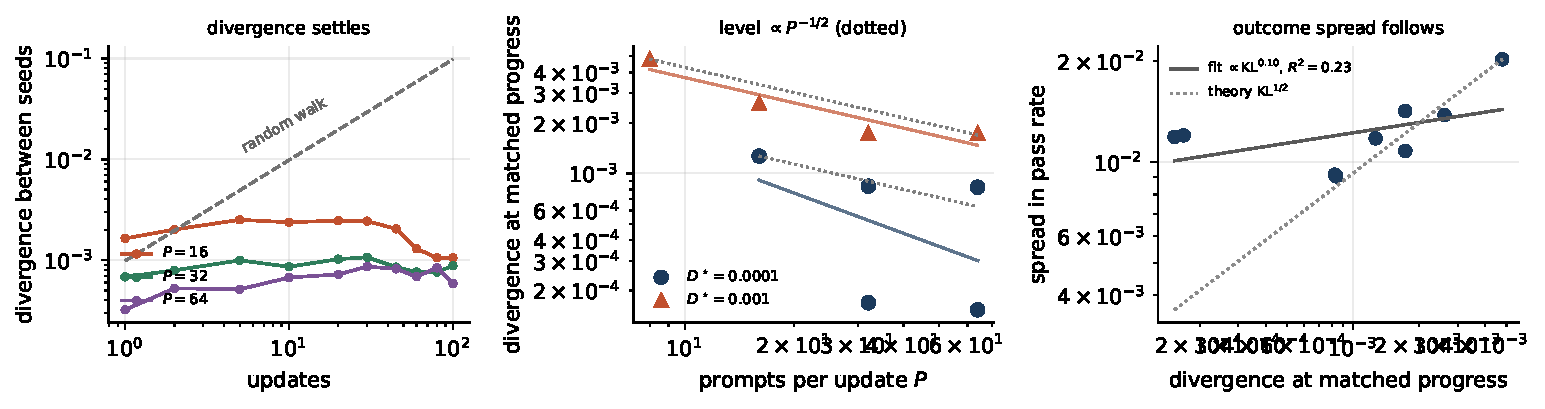
\includegraphics[width=\textwidth]{figures/reconvergence.pdf}
  \caption{\textbf{Left:} divergence between seeds against updates, at a common drift target. The
  dashed line is what an accumulating random walk requires. \textbf{Centre:} the level it settles
  at, compared at matched pass rate rather than matched step count, against the batch; the dotted
  lines are the predicted $P^{-1/2}$. \textbf{Right:} the spread in final pass rate against the
  divergence, one point per setting.}
  \label{fig:reconvergence}
\end{figure*}

\paragraph{It settles.} In every setting that is still learning, divergence rises over the first
few tens of updates and then stops. Fitting a log-log slope over the second half of each run gives
values from $-1.15$ to $+0.26$ across ten settings spanning an eightfold range of batch size and a
tenfold range of drift target, against the $+1$ that accumulation requires. The outcome spread
behaves the same way: it is flat in the number of updates, not growing.

\paragraph{It scales as predicted.} Compared at matched progress, the level follows
$P^{-0.45}D^{0.35}$ against the $P^{-1/2}D^{+1/2}$ of \eqref{eq:seed-scaling}, with $R^2 = 0.94$
over the seven settings where the comparison is available. Both exponents have the right sign and
close to the right magnitude, and the batch is confirmed as the dominant lever: an eightfold
increase in $P$ buys more reproducibility than a tenfold reduction in the step.

\paragraph{What we could not pin down.} \eqref{eq:stationary} factors the level into an injected
noise and a persistence time. The first is measurable; the second is not, at least not the way we
tried. Fitting a single exponential to the approach gives timescales of one to two updates and
predicted levels that miss the measured ones by factors between $1.5$ and $6.6$, with no pattern.
The likely reason is that $H$ has a spectrum rather than one eigenvalue: fast directions equilibrate
immediately and slow ones dominate the final level, so a single-exponential fit is pinned by the
early rise and underestimates what matters. The consequence for practice is a real limitation. The
\emph{scaling} transfers, so a run calibrated once can predict how its reproducibility moves when
the batch or the step changes, which is the question that actually comes up. The absolute level
still requires that one calibration.

\paragraph{Where it stops.} Two of the twelve settings leave the contracting regime, and both do it
the same way. Under a fixed drift target the controller must raise $\eta$ as the signal decays, and
$\E_x[p(1-p)] \to 0$ as a task is solved takes the signal with it. In the two settings that reach a
pass rate above $0.94$, the realised drift runs away to a hundred times its target, divergence jumps
by two orders of magnitude, and the seeds end up in visibly different places: the outcome spread
reaches $0.24$ against $0.01$ elsewhere. This is a failure of drift-targeted control at saturation
rather than of \eqref{eq:stationary}, and it is a caution about a technique we otherwise recommend.

\subsection{Exactly enumerable policies}

The policy is a tabular autoregressive model over a small vocabulary, so its distribution over
sequences, its score at every sequence, and the conditional moments $(p, u_1, S_0, S_1)$ are
available exactly. Propositions~\ref{prop:mean} and~\ref{prop:cov} were checked against
brute-force enumeration over all $|\mathcal{Y}|^{G}$ group outcomes for five estimators and
$G \in \{2,3,4\}$: agreement to $10^{-12}$. The scaled within-prompt term $(G-1)\tr\Sw$, which the
theory treats as $G$-independent, varies by $6\%$ over $G = 2$ to $32$.

\paragraph{The curvature model fails, the drift model does not.} Taking a real update and computing
the resulting improvement and KL exactly, the second-order model of the objective places its optimal
step at least four times below the step that actually maximises improvement, which is where the
sweep ended, because $J = \E[r]$ is
not a log-likelihood and a log-linear policy keeps improving past the turnover of a quadratic model.
The drift model \eqref{eq:drift} predicts the measured KL to between $2.6\%$ and $3.9\%$ across a thousandfold range of step sizes. The theory in Section~\ref{sec:drift} is built on the second of these, not
the first.

\paragraph{Splitting a rollout budget.} For each prompt pool the parameter-free efficiency curve
$\rho(G)$ is compared against the improvement obtained by training at every split of a fixed budget,
holding total rollouts, total drift and step count fixed. Table~\ref{tab:exact-agreement} groups
pools by how much $\rho$ varies across the splits on offer.

\begin{table*}[t]
  \centering
  \begin{tabular}{lccc}
\toprule
predicted spread $\max\rho/\min\rho$ & pools & median $R^2$ & median Spearman \\
\midrule
$1.00$--$1.15$ & 8 & 0.670 & +0.588 \\
$1.15$--$1.35$ & 11 & 0.876 & +0.833 \\
$1.35$--$2.00$ & 6 & 0.971 & +0.957 \\
$2.00$--$8.00$ & 7 & 0.983 & +0.978 \\
\bottomrule
\end{tabular}
  \caption{Agreement between the predicted efficiency and the measured gain in the enumerable
  testbed, as a function of how strongly the prediction discriminates between splits. The prediction
  has no free parameters. Pools where it predicts that the split hardly matters are the pools where
  the measured curves are flat to within their standard errors.}
  \label{tab:exact-agreement}
\end{table*}

\begin{figure*}[t]
  \centering
  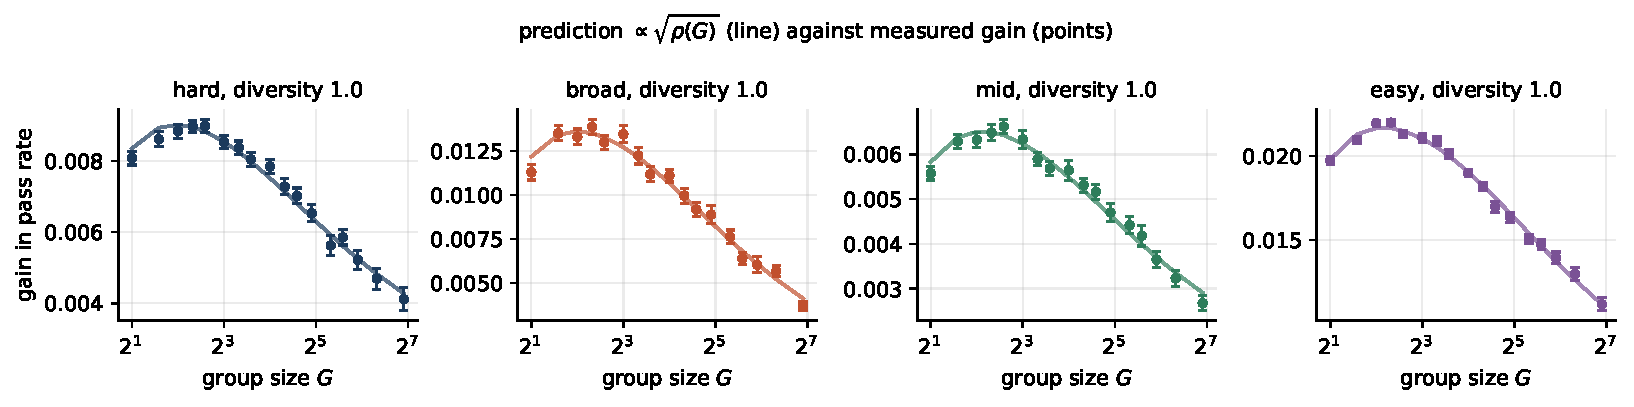
\includegraphics[width=0.98\textwidth]{figures/exact_curves.pdf}
  \caption{Measured gain against $\sqrt{\rho(G)}$ for the four pools whose predictions discriminate
  most strongly. Error bars are standard errors over seeds.}
  \label{fig:exact-curves}
\end{figure*}

\subsection{The estimator}

Figure~\ref{fig:estimator-accuracy} compares the group size recovered by the estimator of
Section~\ref{sec:estimation} against the exactly known value, over pools whose noise ratio spans a
factor of $26$ and whose $G^{\star}$ runs from $3.8$ to $15.2$. The median error in $G^{\star}$ is $1.3\%$
and the worst is $6.2\%$, using $2500$ batches of $32$ prompts split into $K = 8$ blocks; the
individual traces are recovered to $2.1\%$ ($\tau_w$) and $3.4\%$ ($\tau_b$) at the median.

\begin{figure}[t]
  \centering
  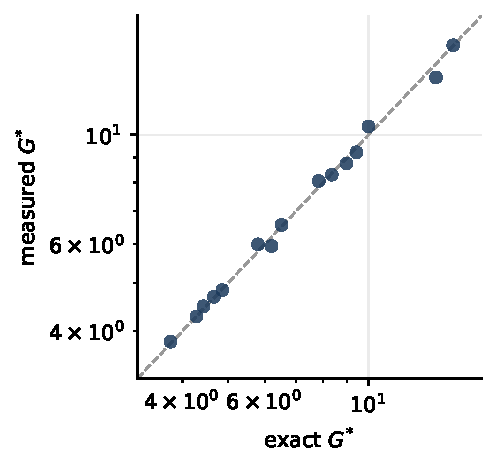
\includegraphics[width=0.92\linewidth]{figures/estimator_accuracy.pdf}
  \caption{Measured against exact optimal group size across prompt pools.}
  \label{fig:estimator-accuracy}
\end{figure}

\subsection{Transformers trained from scratch}

A population of independent transformers is warmed up on a verifiable running-sum task until each
member reaches a common pass rate, the noise terms are measured at that frozen policy, and every
member is then trained from the same starting point at each split of a fixed rollout budget. The
corpus size is the knob: sampling without replacement from a corpus of $N$ scales the between-prompt
term by $1 - (P-1)/(N-1)$, so shrinking the corpus toward the batch raises $G^{\star}$ without touching
the task.

\begin{table*}[t]
  \centering
  \begin{tabular}{lcccccc}
\toprule
corpus $N$ & $\tau_b$ & $\tau_w$ & predicted $G^{\star}$ & best measured $G$ & Spearman & $R^2$ \\
\midrule
128 & 32.1 & 137.1 & 3.38 & 2 & +0.943 & 0.983 \\
192 & 35.4 & 140.3 & 3.17 & 2 & +0.943 & 0.954 \\
512 & 37.6 & 146.8 & 3.04 & 2 & +0.943 & 0.987 \\
4096 & 37.7 & 141.8 & 2.95 & 4 & +1.000 & 0.984 \\
unbounded & 37.3 & 140.0 & 2.94 & 4 & +1.000 & 0.985 \\
\bottomrule
\end{tabular}
  \caption{Predicted and measured optimum on transformers trained from scratch. The sweep visits
  $G \in \{2, 4, 8, 16, 32, 64\}$, so a predicted optimum near three can only appear as a peak at
  two or four; those two are within one standard error of each other in four of the five corpora,
  and every corpus shows the predicted decline beyond $G = 8$. Spearman and $R^2$ are computed
  against the parameter-free prediction across the whole sweep.}
  \label{tab:transformer}
\end{table*}

\begin{figure*}[t]
  \centering
  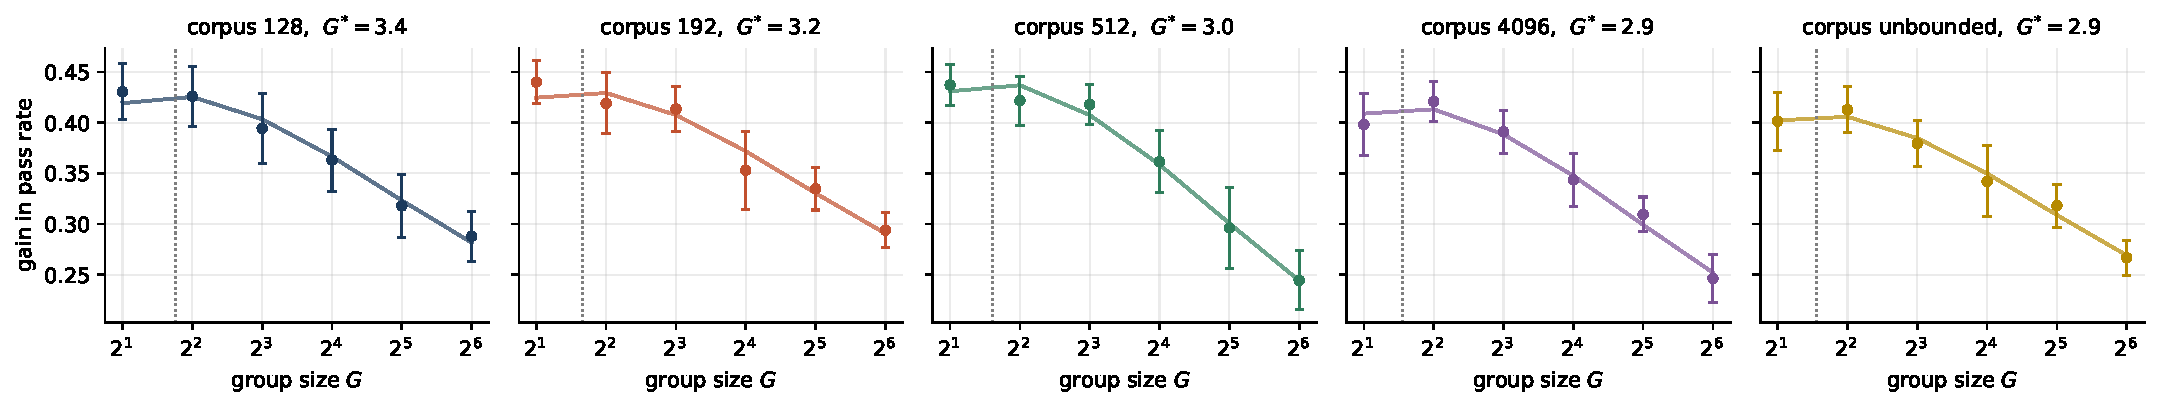
\includegraphics[width=\textwidth]{figures/transformer_curves.pdf}
  \caption{Gain against group size at a fixed rollout budget, with the parameter-free prediction
  overlaid and the predicted $G^{\star}$ marked.}
  \label{fig:transformer-curves}
\end{figure*}

\subsection{Under Adam}
\label{sec:adam}

Everything above is under plain gradient ascent, where the update is the gradient and the noise can
be read in the parameter metric. Real runs use Adam, which moves in a different metric and is scale
invariant, so the theory only carries over if the noise is measured after preconditioning. Repeating
the sweep under both optimisers gives Table~\ref{tab:adam}.

\begin{table*}[t]
  \centering
  \begin{tabular}{lcccccccc}
\toprule
gain by group size & 2 & 4 & 8 & 16 & 32 & 64 & measured $G^{\star}$ & $R^2$ \\
\midrule
gradient ascent & +0.409 & +0.413 & +0.390 & +0.333 & +0.300 & +0.250 & 2.94 & 0.992 \\
Adam & +0.519 & +0.527 & +0.514 & +0.492 & +0.447 & +0.384 & 3.42 & 0.969 \\
\bottomrule
\end{tabular}
  \caption{The same sweep under gradient ascent and under Adam. The optimum is at $G = 4$ for both,
  and the predicted curve explains the measured one about as well. The measured $G^{\star}$ for Adam is
  taken in Adam's own metric, which takes some care -- see below.}
  \label{tab:adam}
\end{table*}

The law survives, but measuring in Adam's metric required fixing two things, and both are
consequences of the preconditioner being an estimated quantity rather than a fixed one.

First, a probe run at a frozen policy starts with an empty second-moment estimate, so there is no
metric to measure in yet. Priming it -- running the optimiser's state forward on real batches with
a zero step size, so the policy does not move -- gives the preconditioner a real run would have.

Second, and less obviously, dividing by $\sqrt{v}$ is unbounded. Coordinates that rarely receive
gradient have a tiny second moment, which is harmless for the update, since Adam's update is
bounded by construction, but ruinous for an inner product between two noisy gradients: those
coordinates dominate it. Measured this way the estimator returned $\tau_b < 0$ and an inverted
efficiency curve. Flooring the second moment at a fraction of its own mean before dividing fixes
it, and the result is insensitive to where the floor is put: over three orders of magnitude in the
floor, the measured $G^{\star}$ moves only from $3.51$ to $3.15$, against an observed optimum of $4$.
Without a floor the same measurement reports $11.9$.

This is the one place where our quantities need care that the plain-gradient case does not. The
working rule is to instrument the update rather than the gradient, and to floor the preconditioner
before inverting it.

\subsection{A pretrained model}

We repeat the measurement on Qwen2.5-0.5B-Instruct with LoRA adapters as the trainable parameters,
over corpora of short exact-match tasks: counting a letter in a word, naming the $k$-th item of a
list, adding two numbers, and a mixture of all of them. Measured optimal group sizes run from $2.7$
to $6.2$, the same range as the enumerable policies and the transformers trained from scratch.

Corollary~\ref{cor:bernoulli} predicts that the within-prompt noise tracks the reward histogram at a
fixed score scale, and difficulty buckets inside one family are where that assumption is tenable.
We screen prompts with a larger sample than the measurement uses, so the bucket boundaries do not
inherit the noise of the quantity under test, and report the pass rate re-measured during the probe
rather than the one used to sort. Across buckets spanning pass rates from $0.25$ to $0.30$, the
ratio $\tau_w/\E[p(1-p)]$ is constant to within $14\%$ (Table~\ref{tab:difficulty}).

\begin{table*}[t]
  \centering
  \small
  \begin{tabular}{lccccc}
\toprule
bucket & screened $p$ & measured $p$ & $\E[p(1-p)]$ & $\tau_w$ & $\tau_w/\E[p(1-p)]$, relative \\
\midrule
0 & 0.160 & 0.253 & 0.163 & 1.15e+04 & 0.90 \\
1 & 0.269 & 0.272 & 0.175 & 1.33e+04 & 0.96 \\
2 & 0.380 & 0.304 & 0.185 & 1.66e+04 & 1.14 \\
\bottomrule
\end{tabular}
  \caption{Within-prompt noise across difficulty buckets of one task family. The gap between the
  screened and re-measured pass rates in the outer buckets is regression to the mean, which is why
  the screening sample is the larger of the two.}
  \label{tab:difficulty}
\end{table*}

Across \emph{different} families the same ratio varies by a factor of $8.8$
(Appendix~\ref{app:cross-family}), and the reason is visible in the assumption: the constant the corollary
predicts is the score scale $\sigma_s^2$, and a family whose answer is one number does not share a
score scale with one whose answer is four. This bounds how the corollary should be used. It
converts a reward histogram into a noise estimate within a task distribution, after one calibration
measurement, and it does not transport that calibration to a task of a different shape.

\subsection{What the hardware is worth}
\label{sec:hardware}

Theorem~\ref{thm:split} turns the split into a question about the serving stack as much as about
the learning problem, through the prefill ratio $\alpha = c_{\mathrm{pre}}/c_{\mathrm{dec}}$. We
measured both costs for a $0.5$B model in bfloat16 on the machine everything else ran on. The ratio
is governed almost entirely by the prompt-to-response length ratio, running from $0.04$ when a
short prompt is followed by a thousand tokens of response to $10.9$ when a thousand-token prompt is
followed by a short answer.

\begin{table*}[t]
  \centering
  \small
  \begin{tabular}{lcccc}
\toprule
$c_{\mathrm{pre}}/c_{\mathrm{dec}}$ & $R=64$ & $R=256$ & $R=1024$ & $R=8192$ \\
\midrule
0.00 & 2.9 & 2.9 & 2.9 & 2.9 \\
0.04 & 3.0 & 3.0 & 3.1 & 4.0 \\
0.70 & 3.6 & 4.0 & 5.5 & 13.1 \\
2.63 & 5.0 & 6.2 & 9.7 & 25.1 \\
10.92 & 8.7 & 11.5 & 19.2 & 51.0 \\
\midrule
\multicolumn{5}{l}{\footnotesize small-batch limit \eqref{eq:gstar-cost} --- $\alpha=0.00$: 2.9, $\alpha=0.04$: 2.9, $\alpha=0.70$: 3.5, $\alpha=2.63$: 4.6, $\alpha=10.92$: 7.6} \\
\bottomrule
\end{tabular}
  \caption{The optimum $G^{\star}$ from Theorem~\ref{thm:split}, at the noise ratio measured on our
  transformers, across measured prefill ratios and rollout budgets. Entries are the root of
  \eqref{eq:stationary}, which agrees with direct numerical minimisation of \eqref{eq:objective} to
  one part in $10^{7}$. The last row shows the small-batch limit, which is what one would quote
  from \eqref{eq:gstar-cost} alone and which understates the optimum badly at large $R$.}
  \label{tab:optimum}
\end{table*}

\begin{figure}[t]
  \centering
  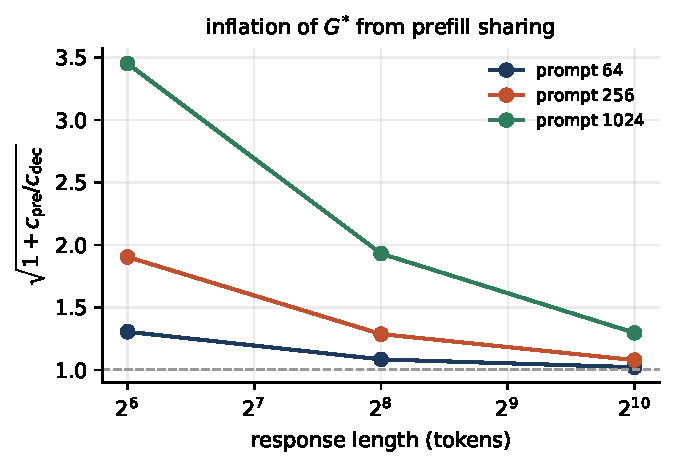
\includegraphics[width=\linewidth]{figures/cost_model.pdf}
  \caption{Measured prefill-to-decode economics on an Apple M4, as the group-size inflation implied
  in the small-batch limit. Long responses make prefill sharing almost worthless; short answers
  behind long prompts make it decisive.}
  \label{fig:cost-model}
\end{figure}

Table~\ref{tab:optimum} is the reconciliation the paper has been building towards. A purely
statistical reading of the split says three; the settings in which published recipes were developed
say otherwise, and the theorem says how much of that is justified. Long prompts with short answers
at a large batch put the optimum in the tens, which is where the recipes are. Reasoning-length
responses, where the response dwarfs the prompt, put it back at three to four, and there a group of
sixteen is spending most of its budget on responses that a second prompt would have used better.
The disagreement between a recipe and this analysis is therefore not evidence against either: it
identifies the regime the recipe came from.

\subsection{What transfers when the batch size changes}

The sharpest consequence of the drift model is a statement about transfer. A run tuned by learning
rate is tuned in a unit that depends on the batch through $\mathcal{G} + N/P$; a run tuned by drift
is not. Table~\ref{tab:transfer} sweeps both parameterisations at four batch sizes and reports what
it costs to carry the value tuned at the smallest batch to the others.

\begin{table*}[t]
  \centering
  \begin{tabular}{lcccc}
\toprule
prompts per step $P$ & 8 & 16 & 32 & 64 \\
\midrule
best step size $\eta^{*}$ & 0.0417 & 0.0786 & 0.1228 & 0.1615 \\
best drift target $D^{*}$ & 5.06e-03 & 5.29e-03 & 5.15e-03 & 3.98e-03 \\
cost of transferring $\eta$ (\%) & +0.0 & -9.9 & -17.9 & -22.0 \\
cost of transferring $D^{*}$ (\%) & +0.0 & +0.0 & +0.0 & +0.0 \\
\bottomrule
\end{tabular}
  \caption{Transfer across batch size. The learning rate that is optimal at $P = 8$ loses a fifth of
  the achievable gain by $P = 64$; the drift target that is optimal at $P = 8$ remains optimal.}
  \label{tab:transfer}
\end{table*}

\begin{figure*}[t]
  \centering
  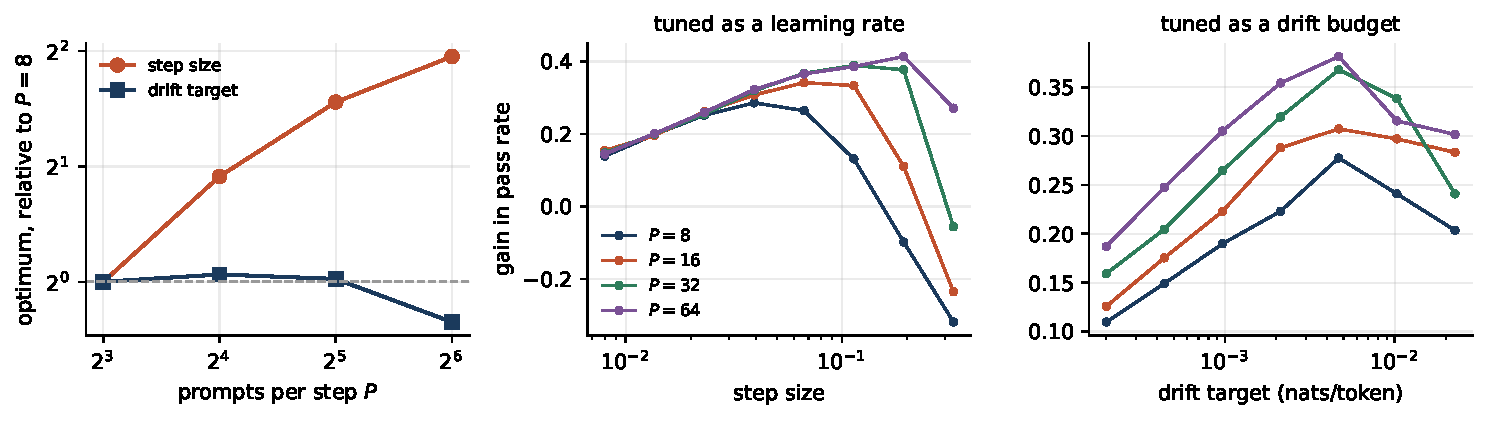
\includegraphics[width=\textwidth]{figures/transfer.pdf}
  \caption{Left: the optimum of each parameterisation relative to its value at $P = 8$. Centre and
  right: the sweeps themselves. The learning-rate optimum moves; the drift optimum does not.}
  \label{fig:transfer}
\end{figure*}

The single-step drift model accounts for part of the movement in $\eta^{*}$ and not all of it: the
coefficient $\mathcal{G} + N/P$ measured at the initial policy predicts a smaller shift than the one
observed over a full run. The coefficient keeps moving as the policy improves, so a controller that re-reads it tracks the
optimum while a learning rate fixed in advance cannot.

\subsection{A prospective test, and where the drift target stops transferring}
\label{sec:recipe}

Everything so far tunes one quantity at a time on the setting it is measured on. The stronger test
is prospective: fix a setting the method has never seen, let the probe choose $G$ before any
training happens, and check afterwards whether it chose well. We moved to a held-out setting with
four times the rollout budget, eight times the corpus and a different seed. The probe reported
$G^{\star} = 3.1$, so the recipe took $G = 4$; the comparison is against $G = 16$, which is what a
default recipe would use.

\begin{table}[t]
  \centering
  \small
  \begin{tabular}{lcc}
\toprule
best achievable gain & $G = 4$ & $G = 16$ \\
\midrule
tuning a learning rate & +0.4947$^{\ast}$ & +0.4780$^{\ast}$ \\
tuning a drift target & +0.4431 & +0.3989 \\
predicted efficiency $\rho$ & 0.815 & 0.674 \\
\bottomrule
\end{tabular}
  \caption{Best achievable gain at the held-out setting, crossing the group size the probe selected
  against the group size a default recipe would use, under both ways of setting the step. Starred
  entries sit at the edge of their grid and are lower bounds. The probe's choice wins under both.}
  \label{tab:diagnosis}
\end{table}

\textbf{The prospective choice was right.} $G = 4$ beats $G = 16$ under both parameterisations.
Under drift control, where the step size is held to the same behavioural budget in both arms and so
cannot confound the comparison, it wins by $11.1\%$ against a predicted
$\sqrt{\rho_4/\rho_{16}} - 1 = 10\%$.

\textbf{The drift target transfers across the group size exactly.} Both group sizes put their
optimum at the same drift target, $1.45 \times 10^{-3}$. Changing how the budget is split does not
change how far the policy should move per update, which is what a behavioural unit ought to do.

\textbf{It does not transfer across this change of budget.} The tuning setting's optimum was
$3.19 \times 10^{-3}$, a factor of $2.2$ away, and carrying it over costs $20\%$ of the achievable
gain. Earlier the same target held to within $5\%$ across a fourfold change in batch size and
$21\%$ across an eightfold one. A sixteenfold change in prompts per step, combined with a fourfold
change in rollout budget, is past where a single number holds. We found this the hard way: packaging
the two together and carrying both to the held-out setting lost to the default by $28.9\%$ (paired
$t = -3.01$ over $32$ runs), and Table~\ref{tab:diagnosis} is what attributes that loss to the drift
target rather than to the group size.

\textbf{A constant drift target is not the right schedule.} At both group sizes a tuned constant
learning rate beat the best constant drift, with its optimum at the edge of the grid. A fixed
learning rate produces a drift that changes over a run as the gradient statistics change, and that
this wins says the optimal drift trajectory is not flat. The unit appears to be right and the
schedule is not, which is the most concrete thing this paper leaves open.
